\documentclass{article}
\usepackage[utf8]{inputenc}

% Paper layout
\setlength{\paperheight}{11in}
\setlength{\paperwidth}{8.5in}
\oddsidemargin 0.0in 
\evensidemargin .5in
\marginparwidth 0.07 true in
\textheight 7.5 true in
\textwidth 6.5 true in 

\PassOptionsToPackage{numbers, compress}{natbib}
\usepackage{url}
\usepackage{graphicx}
\usepackage{parskip}
\usepackage{mathtools}
\usepackage{fancyvrb}
\usepackage{array,booktabs,calc,blindtext}
% \usepackage[shortlabels]{enumerate}

%%%%%%%%%%%%%%%%%%%%%%%%%%%%%%%%%%%%%%%%%%%%%%%%%%%%%%%%%%%%%%%%%%%%%%%%%%%%%%%%

\newcommand{\hmwkTitle}{Extensible Physics Engine}
% \newcommand{\hmwkIssueDate}{22 February 2017}
\newcommand{\hmwkDueDate}{8 May 2017}
\newcommand{\hmwkClass}{6.905/6.945 Final Project Draft}
% \newcommand{\hmwkClassInstructor}{Professor Gerry Sussman}
\newcommand{\hmwkAuthorName}{\textbf{Michael Chang, Abigail Choe, Leon Shen}}

\title{
    \textmd{\hmwkClass:\ \hmwkTitle}\\
    % \normalsize{\hmwkClassInstructor}\\
    % \small{Issued\ on\ \hmwkIssueDate}\\
    \small{Due\ on\ \hmwkDueDate}
}
\author{\hmwkAuthorName}
\date{}
\begin{document}
\maketitle
\section{Introduction}

Physics can be viewed as the programming language of the natural world. From
quantum mechanics to Newtonian mechanics to relativistic mechanics, the
theories at these different levels of explanation each describe their
primitives, means of combination, and means of abstraction over objects,
relations, and events. Physical particles, objects, and entities are data, and
the laws that govern how they evolve over time are procedures that operate on
this data.  

Our project aims to explore this view by implementing a simple physics engine
in scheme. We designed the physics engine to be generic and extensible. For
example, it is very straightforward to define new worlds on the underlying
substrate as well as to define new objects and forces within a given world.
This paper presents the design of the infrastructure for the physics engine,
describes how objects and forces can be easily defined and added on top of the
infrastucture, and illustrate several demonstrations of the system on worlds
with gravitational and electrostatic forces.

% motivation: features of physics engine that incorporate ideas from class (e.g.
% generic operator, hierarchy, propagator, language for language (high--low)),
% cool visualization of concepts from class

\section{Infrastructure}

We used the object system from pset 4 to model physical objects in our
simulated world, as well as the world itself. Having the ability to create a
hierarchy of types allows us to derive new types of physical objects to be
simulated from previously defined types (see section Object Types).

% internal NOTE: generic procedures--we haven't actually used them in the code yet!

% NOTE: feel like this should be merged with object types and arithmetic

% what we did, how we did it, why we did it

\section{Arithmetic}

We incorporated the generic arithmetic developed in pset 3. We extended the
vector-arithmetic to support element-wise operations between scalars and
vectors. We did this by coercing scalars to become vectors that contain the
same value. For example, \texttt{(+ \#(3 4) 1)} gets transformed into
\texttt{(+ \#(3 4) \#(1 1))}. 

This extension was made to allow our system to operate on any $n$th dimension
vector, and therefore be applicable to any $n$th dimension world
representation. For example, though the examples in this paper concern 2-dimensional worlds, the physics can easily be extended to 3-dimensinoal worlds. The default velocity of an object is set to 0 if it is not
specified. Supporting arithmetic operations between a scalar and a vector
enables our system to use a single default value 0 that is compatible with any
vector instead of limiting our system to the dimension of the default zero
vector specified.  

The coercion method is 
\begin{verbatim}
(define (coerce a size-reference)
  (if (vector? a)
    a
    (make-vector (vector-length size-reference) a)))
\end{verbatim}

The rest of the infrastructure for generic procedures was adapted from pset 4,
but pset 4's generic arithmetic is not compatible with that of pset 3. To fix
this issue, we first loaded the relevant pset 3 dependencies, installed a
generic arithmetic with vector operations, redefined arithmetic operations to
be the ones from that generic arithmetic (such as with \texttt{(define *
(access * arith-environment))}), and then loaded the pset 4 generic procedure
infrastructure on top.

\section{Physics Engine}
\subsection{Object Types}

There are three types of objects in the system: \texttt{thing}, \texttt{interaction}, and \texttt{world}. \texttt{thing} refers to all physical objects in the system. There is a hierarchy of physical objects that have additional properties. For example, type \texttt{point-charge} has an additional property \texttt{charge} and experiences electric forces while type \texttt{ball} experiences only gravity. Each \texttt{thing} keeps a list of \texttt{interaction} that is used to update itself. \texttt{interaction} refers to forces exerted on \texttt{thing}s. \texttt{interaction} includes a procedure that calculates the force as well as \texttt{influences}, a list of \texttt{thing}s that contribute to that force. Similar to \texttt{thing}, subtypes of \texttt{interaction}s form a hierarchy. Lastly, \texttt{world} keeps a list of all \texttt{thing}s and an \texttt{update} call to the \texttt{world} calls on each \texttt{thing} to update itself.

% (subject to change after restructuring)

\subsection{Updating Physical Objects}

There are mainly two ways positions of physical objects could be updated: 1)
The evolver can take in a list of forces and objects and apply forces as
appropriate 2) Each object can be registered with a set of forces applicable to
it and the evolver can call each object to evolve itself.

Our system adopted the second model where each object updates itself. This
model makes it easier to handle different types of forces exerted on specific
types of object. Moreover, in the second model, the engine does not need to be
notified and updated everytime a new object is added. Instead, update or
addition of new \texttt{interaction}s is taken care of at the object level when
it is added.

% (TODO: add eval/apply code after restructuring)

\subsection{Output Display}

Our engine updates each object every timestep and re-renders them on the
screen:

\begin{verbatim}
(define (run-engine world steps)
  (reset-graphics)
  (if (> steps 0)
    (begin 
      (for-each 
        (lambda (thing)
            (newline)
            (display (cons (get-name thing) (get-position thing)))  ; for debugging
            (render thing))
        (get-world-all-things world))
      (update-world world)
    (run-engine world (- steps 1)))))
\end{verbatim}

where the \texttt{render} procedure takes in a \texttt{thing}, checks what type
of thing it is, and renders the object appropriately.

\section{Demos}
\subsection{Gravity}
% \begin{samepage}

We can easily extend our system with new forces and new objects. We begin by
creating an gravity as an \texttt{interaction}:

{\small\begin{verbatim}
(define (make-gravity thing all-things)
  (define (procedure thing influences)
    (sum (map (lambda (influence)
                (let* ((m1 (get-mass thing))
                       (m2 (get-mass influence))
                       (G 6.674e-11)
                       (v (- (get-position influence)  ; vector between influence and thing
                            (get-position thing)))
                       (r (magnitude v))               ; distance between influence and thing
                       (u (/ v r))                     ; unit vector
                       (gmag (* (* G m1 m2)            ; magnitude of gravity
                                (/ 1 (square r)))))
                  (* u gmag)))                        ; gravitational force vector
              influences)))
  (let ((influences (delq thing all-things)))
    (make-interaction gravity? 'gravity procedure influences)))
\end{verbatim}}
% \end{samepage}

\begin{figure}[h!]
  \centering
 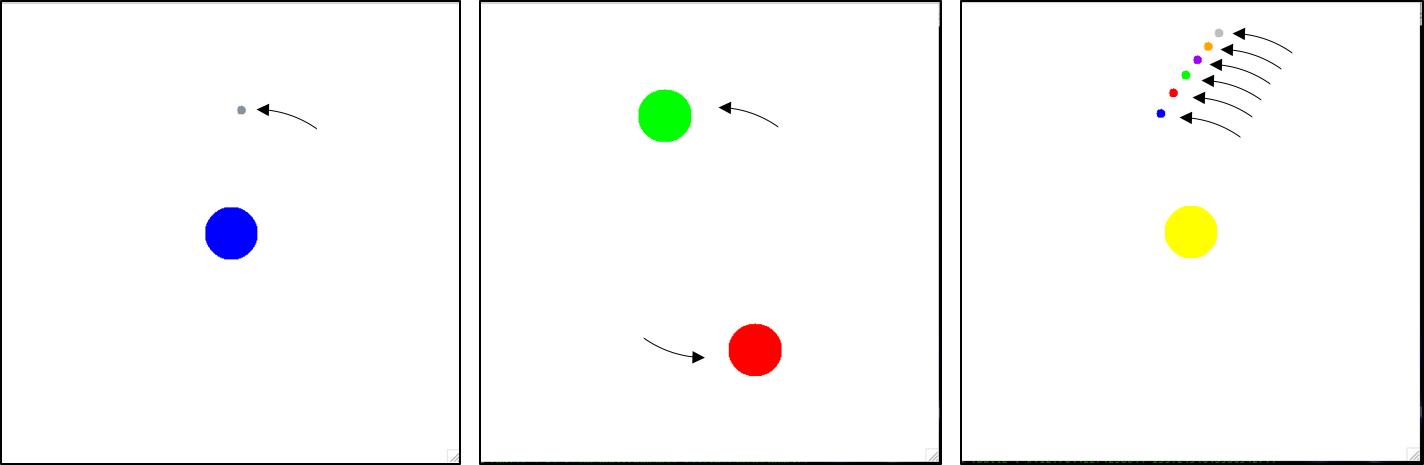
\includegraphics[width=\textwidth,height=\textheight,keepaspectratio]{figs/gravity.png}
  \caption{[\textit{left}] \texttt{earth-moon}; [\textit{center}] \texttt{binary-stars}; [\textit{right}] \texttt{solar-system}}
  \label{figure:gravity}
\end{figure}

We've created several worlds that exhibit gravity (Fig. \ref{figure:gravity}).
Once an object is added to the world, any object that has mass will feel
gravitational forces with other object that have mass.

% \begin{samepage}
This world contains an earth with a moon orbiting around it.
{\small\begin{verbatim}
(define (earth-moon)
  (define w (make-world "world"))
  (define b1 (make-ball "earth" 30 1e15 #(0 0) #(0 0) "blue"))
  (define b2 (make-ball "moon" 5 1e5 #(100 100) #(-15.361 15.361) "#85929E"))

  (add-mass! b1 w)
  (add-mass! b2 w)
  w)
\end{verbatim}}
% \end{samepage}

% \begin{samepage}

This world contains two equal masses orbiting a common center of mass.

{\small\begin{verbatim}
(define (binary-stars)
  (define w (make-world "world"))
  (define b1 (make-ball "ball1" 5 1e15 #(-100 -100) #(9 -9) "red"))
  (define b2 (make-ball "ball2" 5 1e15 #(100 100) #(-9 9) "green"))

  (add-mass! b1 w)
  (add-mass! b2 w)
  w)
\end{verbatim}}
% \end{samepage}

% \begin{samepage}

This world contains a massive sun and several planets orbitting around the sun.

{\small\begin{verbatim}
(define (solar-system)
  (define w (make-world "world"))
  (define s (make-ball "sun" 30 1e15 #(0 0) #(0 0) "yellow"))
  (define b1 (make-ball "ball1" 5 1e5 #(100 100) #(-15.361 15.361) "blue"))
  (define b2 (make-ball "ball2" 5 1e5 #(110 110) #(-15.361 15.361) "red"))
  (define b3 (make-ball "ball3" 5 1e5 #(120 120) #(-15.361 15.361) "green"))
  (define b4 (make-ball "ball4" 5 1e5 #(130 130) #(-15.361 15.361) "purple"))
  (define b5 (make-ball "ball5" 5 1e5 #(140 140) #(-15.361 15.361) "orange"))
  (define b6 (make-ball "ball6" 5 1e5 #(150 150) #(-15.361 15.361) "gray"))

  (add-mass! s w)
  (add-mass! b1 w)
  (add-mass! b2 w)
  (add-mass! b3 w)
  (add-mass! b4 w)
  (add-mass! b5 w)
  (add-mass! b6 w)
  w)
\end{verbatim}}
% \end{samepage}

\subsection{Electromagentism}
% \begin{samepage}

Let's add electric forces between point charges into the physics engine.

{\small\begin{verbatim}
(define (make-electric-force point-charge all-point-charges)
  (define (procedure point-charge influences)
    (sum (map (lambda (influence)
                (let* ((q1 (get-point-charge-charge point-charge))
            		       (q2 (get-point-charge-charge influence))
            		       (epsilon0 8.854e-12) ; vacuum permittivity
                       ;; vector between influence and point charge
            		       (v (- (get-position influence)
                             (get-position point-charge)))
                       ;; distance between influence and point charge
            		       (r (magnitude v))
                       ;; unit vector * -1 to account for opposite signs
                       ;; attract & same signs repel
            		       (u (* -1 (/ v r)))
            		       (melec (/ (* q1 q2)  ; magnitude of electric force
                                 (* 4 pi epsilon0 (square r)))))
                  (* u melec))) ; multiply unit vector by magnitude of force
              influences)))
  (let ((influences (delq point-charge all-point-charges)))
    (make-interaction electric-force? 'electric-force procedure influences)))
\end{verbatim}}
% \end{samepage}

% \begin{samepage}

This is a simple world with two point charges repelling each other.

{\small\begin{verbatim}
(define (charges-1)
  (define w (make-world "world"))
  (define m1 (make-point-charge "charge1" 1e-3 1 #(-30 -30) #(0 0) "red"))
  (define m2 (make-point-charge "charge2" 1e-3 1 #(30 30) #(0 0) "red"))

  (add-point-charge! m1 w)
  (add-point-charge! m2 w)
  w)
\end{verbatim}}
% \end{samepage}

% \begin{samepage}

This world contains two positively charged masses (blue) and two negatively
charged masses (red).

{\small\begin{verbatim}
(define (charges-2)
  (define w (make-world "world"))
  (define m1 (make-point-charge "charge1" 1e-3 1 #(-100 -100) #(0 0) "red"))
  (define m2 (make-point-charge "charge2" -1e-3 1 #(100 100) #(0 0) "blue"))
  (define m3 (make-point-charge "charge3" 1e-3 1 #(-100 100) #(0 0) "red"))
  (define m4 (make-point-charge "charge4" -1e-3 1 #(100 -100) #(0 0) "blue"))

  (add-point-charge! m1 w)
  (add-point-charge! m2 w)
  (add-point-charge! m3 w)
  (add-point-charge! m4 w)
  w)
\end{verbatim}}
% \end{samepage}

% \begin{samepage}

We can also combine gravity and electric charge. Here, we created a solar-system-like world where each of the planets repel each other and the sun attracts the planets via gravity and electric force. As figure \ref{figure:charges} (right) shows, this charged solar system exhibits wider and diverging orbits compared to figure \ref{figure:gravity} (right), the solar system with only gravity.

{\small\begin{verbatim}
(define (charged-solar-system)
  (define w (make-world "world"))
  (define s (make-point-charge "sun" 3e-3 1e15 #(0 0) #(0 0) "blue"))
  (define b1 (make-point-charge "ball1" -1e-1 1e5 #(100 100) #(-15.361 15.361) "red"))
  (define b2 (make-point-charge "ball2" -1e-1 1e5 #(110 110) #(-15.361 15.361) "red"))
  (define b3 (make-point-charge "ball3" -1e-1 1e5 #(120 120) #(-15.361 15.361) "red"))
  (define b4 (make-point-charge "ball4" -1e-1 1e5 #(130 130) #(-15.361 15.361) "red"))
  (define b5 (make-point-charge "ball5" -1e-1 1e5 #(140 140) #(-15.361 15.361) "red"))
  (define b6 (make-point-charge "ball6" -1e-1 1e5 #(150 150) #(-15.361 15.361) "red"))

\end{verbatim}}
% \end{samepage}

\begin{figure}[h!]
  \centering
 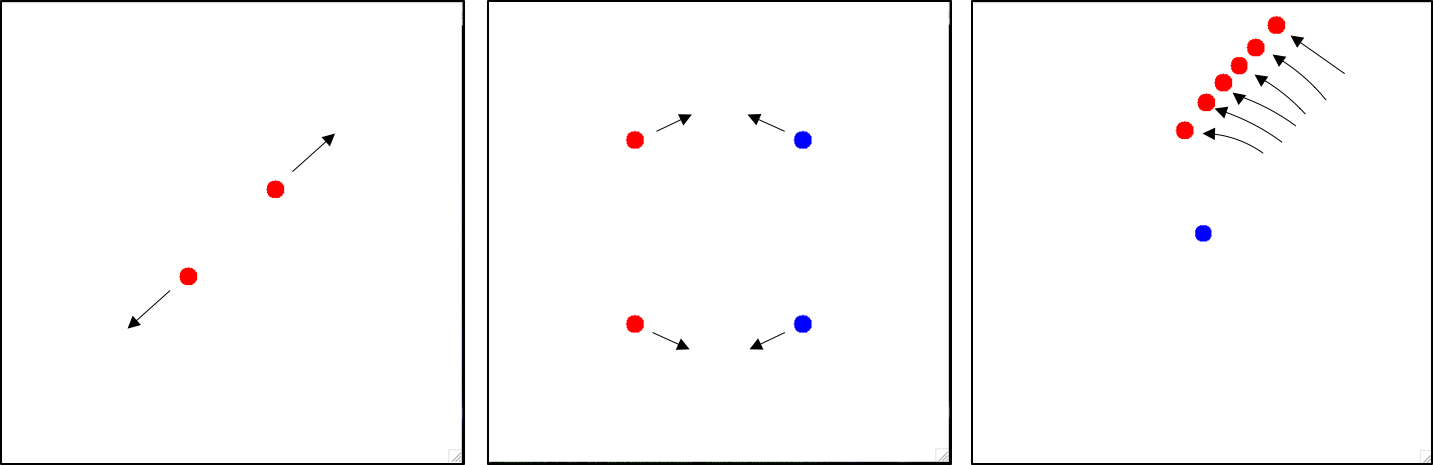
\includegraphics[width=\textwidth,height=\textheight,keepaspectratio]{figs/charges.png}
  \caption{[\textit{left}] \texttt{charges-1}; [\textit{center}] \texttt{charges-2}; [\textit{right}] \texttt{charged-solar-system}}
  \label{figure:charges}
\end{figure}


\section{Extensibility of the System}
Future extensions include collisions between objects, constraints such as joints, simulating objects in three dimensions, and being able to combine objects into larger systems of objects. Collisions and other kinds of constraints could be implemented by adding an interaction that produces forces that enforce these constraints. Objects could be simulated in three dimensions by defining three dimensional object types and using the generic arithmetic to operate on higher dimensional vectors. Objects could be combined into larger systems using procedures, if there is a way to link them together, for example by constraints.

\end{document}
